% Options for packages loaded elsewhere
\PassOptionsToPackage{unicode}{hyperref}
\PassOptionsToPackage{hyphens}{url}
%
\documentclass[
]{article}
\usepackage{amsmath,amssymb}
\usepackage{lmodern}
\usepackage{iftex}
\ifPDFTeX
  \usepackage[T1]{fontenc}
  \usepackage[utf8]{inputenc}
  \usepackage{textcomp} % provide euro and other symbols
\else % if luatex or xetex
  \usepackage{unicode-math}
  \defaultfontfeatures{Scale=MatchLowercase}
  \defaultfontfeatures[\rmfamily]{Ligatures=TeX,Scale=1}
\fi
% Use upquote if available, for straight quotes in verbatim environments
\IfFileExists{upquote.sty}{\usepackage{upquote}}{}
\IfFileExists{microtype.sty}{% use microtype if available
  \usepackage[]{microtype}
  \UseMicrotypeSet[protrusion]{basicmath} % disable protrusion for tt fonts
}{}
\makeatletter
\@ifundefined{KOMAClassName}{% if non-KOMA class
  \IfFileExists{parskip.sty}{%
    \usepackage{parskip}
  }{% else
    \setlength{\parindent}{0pt}
    \setlength{\parskip}{6pt plus 2pt minus 1pt}}
}{% if KOMA class
  \KOMAoptions{parskip=half}}
\makeatother
\usepackage{xcolor}
\IfFileExists{xurl.sty}{\usepackage{xurl}}{} % add URL line breaks if available
\IfFileExists{bookmark.sty}{\usepackage{bookmark}}{\usepackage{hyperref}}
\hypersetup{
  pdftitle={Combining medium-intensity tillage to improve soil compaction and infiltration with cover crop mixes to suppress weeds},
  pdfkeywords={urban, compact, weed, till, cover, water},
  hidelinks,
  pdfcreator={LaTeX via pandoc}}
\urlstyle{same} % disable monospaced font for URLs
\usepackage[margin=1in]{geometry}
\usepackage{longtable,booktabs,array}
\usepackage{calc} % for calculating minipage widths
% Correct order of tables after \paragraph or \subparagraph
\usepackage{etoolbox}
\makeatletter
\patchcmd\longtable{\par}{\if@noskipsec\mbox{}\fi\par}{}{}
\makeatother
% Allow footnotes in longtable head/foot
\IfFileExists{footnotehyper.sty}{\usepackage{footnotehyper}}{\usepackage{footnote}}
\makesavenoteenv{longtable}
\usepackage{graphicx}
\makeatletter
\def\maxwidth{\ifdim\Gin@nat@width>\linewidth\linewidth\else\Gin@nat@width\fi}
\def\maxheight{\ifdim\Gin@nat@height>\textheight\textheight\else\Gin@nat@height\fi}
\makeatother
% Scale images if necessary, so that they will not overflow the page
% margins by default, and it is still possible to overwrite the defaults
% using explicit options in \includegraphics[width, height, ...]{}
\setkeys{Gin}{width=\maxwidth,height=\maxheight,keepaspectratio}
% Set default figure placement to htbp
\makeatletter
\def\fps@figure{htbp}
\makeatother
\setlength{\emergencystretch}{3em} % prevent overfull lines
\providecommand{\tightlist}{%
  \setlength{\itemsep}{0pt}\setlength{\parskip}{0pt}}
\setcounter{secnumdepth}{-\maxdimen} % remove section numbering
\newlength{\cslhangindent}
\setlength{\cslhangindent}{1.5em}
\newlength{\csllabelwidth}
\setlength{\csllabelwidth}{3em}
\newlength{\cslentryspacingunit} % times entry-spacing
\setlength{\cslentryspacingunit}{\parskip}
\newenvironment{CSLReferences}[2] % #1 hanging-ident, #2 entry spacing
 {% don't indent paragraphs
  \setlength{\parindent}{0pt}
  % turn on hanging indent if param 1 is 1
  \ifodd #1
  \let\oldpar\par
  \def\par{\hangindent=\cslhangindent\oldpar}
  \fi
  % set entry spacing
  \setlength{\parskip}{#2\cslentryspacingunit}
 }%
 {}
\usepackage{calc}
\newcommand{\CSLBlock}[1]{#1\hfill\break}
\newcommand{\CSLLeftMargin}[1]{\parbox[t]{\csllabelwidth}{#1}}
\newcommand{\CSLRightInline}[1]{\parbox[t]{\linewidth - \csllabelwidth}{#1}\break}
\newcommand{\CSLIndent}[1]{\hspace{\cslhangindent}#1}
\usepackage{booktabs}
\usepackage{longtable}
\usepackage{array}
\usepackage{multirow}
\usepackage{wrapfig}
\usepackage{float}
\usepackage{colortbl}
\usepackage{pdflscape}
\usepackage{tabu}
\usepackage{threeparttable}
\usepackage{threeparttablex}
\usepackage[normalem]{ulem}
\usepackage{makecell}
\usepackage{xcolor}
\ifLuaTeX
  \usepackage{selnolig}  % disable illegal ligatures
\fi

\title{Combining medium-intensity tillage to improve soil compaction and infiltration with cover crop mixes to suppress weeds}
\author{true \and true \and true}
\date{}

\begin{document}
\maketitle
\begin{abstract}
Urban soils have been degraded by decades of industrial activities, but they also represent opportunities to improve food sovereignty for urban residents practicing urban agriculture.
Urban growers often rely on independent strategies of compost, tillage, or cover cropping, without distinguishing each's distinct benefits, ultimately informing an integrated approach.
This study examined how tillage methods representing various intensities and cover crop mixes targeting different functions affected agricultural variables including soil compaction, water infiltration rate, herbaceous weedy plant pressure, and crop yield.
Results showed that tractor-till significantly relieved compaction in deeper soils compared to roto-till, followed by roto-till compared to no-till.
However, roto-till showed the fastest infiltration and tractor-till allowed the densest weeds, challenging ubiquitous use of tractor-till for urban agriculture.
Results also showed that the mix of sorghum-sudangrass, buckwheat, and cowpea significantly reduced weed density and richness compared to all other mixes, and that the perennial plant mix significantly affected compaction, but without affecting soil water infiltration rates.
Despite theses differences, radish yield was not yet affected by tillage.
Overall, this study further informs urban soil agricultural management by analyzing specific benefits of common methods, advocating an integrated approach including both roto-till for compaction relief and water infiltration benefit, and mixed cover cropping for weed suppression.
\end{abstract}

{
\setcounter{tocdepth}{2}
\tableofcontents
}
Journals:
- Elsevier--Soil \& Tillage Research (IF=5, Elsevier),
\emph{- Land Degradation \& Development (Research vs.~Original, IF=5, Wiley), }
\emph{- Urban Forestry \& Urban Greening (1wk), or then {[}Wiley--{]}}
- ASA Agronomy Journal (?),
- Ecology \& Evolution (replicates), or lastly
- PCI Ecology submission (45d) w/
- pre-print archived in agriRxiv, ecoEvoRxiv, or bioRxiv.

\hypertarget{introduction}{%
\section{Introduction}\label{introduction}}

Urban soils have the potential to improve the livelihoods of most of the world \emph{(\protect\hyperlink{ref-ref}{\textbf{ref?}})} via implications for climate adaptation, erosion and storm-water runoff management, and local forestry \emph{(\protect\hyperlink{ref-payao-zuckerman08}{\textbf{payao-zuckerman08?}})}, but many urban soils are in poor health for cultivation after decades of industrial use, including sealing and structural engineering \emph{(\protect\hyperlink{ref-oldeman91}{\textbf{oldeman91?}})}.
This is especially notable in post-industrial cities of the mid-western USA, where many vacant lots remain on soils can have relatively high compaction, pH, and chemical contamination \emph{(\protect\hyperlink{ref-beniston11}{\textbf{beniston11?}})}.
Degraded urban soils with low organic matter are also likely far from organic carbon saturation \emph{(\protect\hyperlink{ref-stewart07}{Stewart et al. 2007})}, making the potential response to tailored agricultural management large \emph{(\protect\hyperlink{ref-kumar16}{Kumar and Hundal 2016}; \protect\hyperlink{ref-kuzyakov19}{Kuzyakov and Zamanian 2019})}.
However, popular single strategies like organic compost amendments to urban gardens, while widely beneficial across many physical, chemical, and biological properties \emph{(\protect\hyperlink{ref-refs}{\textbf{refs?}})}, can also have other side effects like excess phosphorus \emph{(\protect\hyperlink{ref-small19}{Small et al. 2019})}, which highlights the benefits of new and ongoing research studies of urban soil management, especially of integrated approaches for soil multifunctionality \emph{(\protect\hyperlink{ref-blesh17}{\textbf{blesh17?}})} including cover cropping, tillage, diverse mulching, and others.
In response to various needs, urban agriculture continues to expand as local communities and non-profit organizations revitalize and establish a diversity of new green initiatives including landscaping to improve local access to healthy food and a cleaner and safer environment \emph{(\protect\hyperlink{ref-heckler12}{\textbf{heckler12?}})}.
Urban growers in particular often invest relatively large amounts of money, time, and resources from accessible capital into amending soils for vegetable production \emph{(\protect\hyperlink{ref-ref}{\textbf{ref?}})},
thereby improving the potential impact of research for promising accessible urban soil remediation strategies, which remains limited beyond compost \emph{(\protect\hyperlink{ref-ref}{\textbf{ref?}})}.

Mechanized tilling has long been a regular strategy improve short-term arability, among others like adding compost, although research studies increasingly report soil degradation after long-term and intensive tillage.
Short-term tillage benefits include larger soil pores and lower soil bulk density \emph{(\protect\hyperlink{ref-hill85}{\textbf{hill85?}}; \protect\hyperlink{ref-badalikova09}{\textbf{badalikova09?}})}, and more available nutrients \emph{(\protect\hyperlink{ref-ref}{\textbf{ref?}})} yet less weed regeneration \emph{(\protect\hyperlink{ref-ref}{\textbf{ref?}})}, making tillage useful against soil compaction and associated water infiltration and drainage issues, which facilitates faster seeding and crop establishment early in the season \emph{(\protect\hyperlink{ref-ref}{\textbf{ref?}})}.
However, longer-term side effects of excessive and/or very intensive tillage include weaker soil aggregate stability \emph{(\protect\hyperlink{ref-six99}{\textbf{six99?}})} and structure \emph{(\protect\hyperlink{ref-catania18}{\textbf{catania18?}})}, increasing dependence on tillage to maintain past yields \emph{(\protect\hyperlink{ref-ref}{\textbf{ref?}})}, \ldots{}\emph{(\protect\hyperlink{ref-ref}{\textbf{ref?}})} and faster soil erosion \emph{(\protect\hyperlink{ref-handelsman21}{\textbf{handelsman21?}})}, which has more recently led to events like the USA Dust Bowl \emph{(\protect\hyperlink{ref-ref}{\textbf{ref?}})}, and historically poses an existential threat to agricultural societies when combined with other stressors \emph{(\protect\hyperlink{ref-montgomery07}{Montgomery 2007}; \protect\hyperlink{ref-amundson20}{\textbf{amundson20?}})}.
In response, sustainable and regenerative agriculture movements advise no-till or minimal-till management approaches, like broadfork tools, to re-focus on soil health and fertility \emph{(\protect\hyperlink{ref-xiao-bin06}{\textbf{xiao-bin06?}}; \protect\hyperlink{ref-roger-estrade10}{\textbf{roger-estrade10?}})}, which comes with different challenges like stronger pressure from weeds \emph{(\protect\hyperlink{ref-ref}{\textbf{ref?}})}, highlighting a role for continuing research into diverse no-till strategies.
For urban growers, machinery can also be cost-prohibitive, and limited access to agricultural loans \emph{(\protect\hyperlink{ref-USDA}{\textbf{USDA?}})} has resulted in affected communities adapting by organizing equipment sharing systems, which can be more practical in denser urban housing arrangements compared to diffuse rural ones.
This variation in accessibility of machinery can promote mixed tillage strategies by urban growers including tractor- and/or roto-till, which likely have different effects on soil and weed issues, but there remains little public documentation comparing benefits of various tillage styles on remediating urban soils \emph{(\protect\hyperlink{ref-ref}{\textbf{ref?}})}, which slows the innovation of tailored management strategies for the array of urban grower goals.

Cover cropping has been another long-recommended strategy of sustaining longer-term yields by maintaining soil fertility \emph{(\protect\hyperlink{ref-carverux2fwhite}{\textbf{carver/white?}}; \protect\hyperlink{ref-handelsman}{\textbf{handelsman?}})}, although current strategies could be improved from relying on single species to designing complementary species mixes.
The namesake benefit of cover crops is to cover the soil in areas without active cultivation, which maintains root activity and weakens erosion \emph{(\protect\hyperlink{ref-ref}{\textbf{ref?}})}, but different species will also vary in the benefits they can provide based on physiological traits.
For example, legumes like cowpea (or black-eyed peas, \emph{Vigna unguiculata}), clovers (\emph{Trifolium sp.}), and hairy vetch (\emph{Vicia villosa}) are popular cover crops because of their additional symbioses with root bacteria that fix nitrogen from the air into soils where it is more available for future crop use \emph{(\protect\hyperlink{ref-grossman}{\textbf{grossman?}})}.
Similarly, buckwheat helps scavenge soil phosphorus \emph{(\protect\hyperlink{ref-SAREguide}{\textbf{SAREguide?}})}, which is often a limiting macro-nutrient in the tropics \emph{(\protect\hyperlink{ref-ref}{\textbf{ref?}})}, and could also be combined with compost that is usually high in phosphorus to address a recurring soil phosphorus deficiency.
Other plants, including grasses like sorghum, tend to grow deep roots, or have other traits like chemical defenses named allelopathy, that compete with weeds enough to keep them suppressed over time \emph{(\protect\hyperlink{ref-SAREguide}{\textbf{SAREguide?}})}.
Broader implications of cover cropping also include higher soil organic matter, though the underlying processes remain complex \emph{(\protect\hyperlink{ref-king20}{\textbf{king20?}})}, and few studies show direct correlations \emph{(\protect\hyperlink{ref-oldfield19}{Oldfield, Bradford, and Wood 2019})}.
Furthermore, while large rural organic farms can benefit from incorporating specifically-chosen cover cropping into their mechanized operations, the reliance of urban agriculture more on labor over machinery offers an opportunity to develop new cover cropping systems that combine seeding and terminating different species together to improve the potential efficiency of soil remediation efforts.
For example, sorghum, cowpea, and buckwheat could be combined into a mixed strategy that can increase soil nitrogen, soil phosphorus, and suppress weeds via deep and shallow roots with allelopathic chemical defenses, although cover crop synergisms remain understudied \emph{(\protect\hyperlink{ref-ref}{\textbf{ref?}})}.
An integrated complex approach to optimizing cover cropping systems including interspecific species interactions are well-posed to be initially researched in urban agriculture and followed by later adaptation to rural agriculture as well \emph{(\protect\hyperlink{ref-nationalSciTechCouncil17}{\textbf{nationalSciTechCouncil17?}})}.

In this study, we investigated how different tillage techniques and cover crop species mixes affect soil physical properties and yield {[}over the course of one growing season{]}.
The tillage methods ranged from high disturbance using a tractor and implements to minimal disturbance with a broadfork.
Cover crop species mixes were selected based on target functions including reducing compaction, suppressing weeds, and perenniality, or potential for sustainable re-growth.
We hypothesized that the benefits of tillage and cover crop mixing would be interchangeable, meaning that both tillage and cover crop mixes could improve soil compaction and suppress weeds to similar degrees, also increasing yield.
Accordingly, we predicted that roto-till, a moderate soil disturbance, would best balance compaction and weed pressure benefits, deepening where soil hardpan layers occur that limit root penetration, increasing soil water infiltration rates, and reducing weed cover, density, and diversity.
We also expected that the cover crop mix designed against soil compaction would have the deepest soil harpan depth and highest water infiltration rates compared to other mixes, due to the strong rooting by selected radish and ryegrass species.
Finally we expected that the cover crop mix designed for weed suppression would experience the lowest local weed cover, density, and diversity, due to allelopathic chemical defense traits.

\hypertarget{methods}{%
\section{Methods}\label{methods}}

\begin{verbatim}
## -- Attaching packages --------------------------------------- tidyverse 1.3.1 --
\end{verbatim}

\begin{verbatim}
## v ggplot2 3.3.6     v purrr   0.3.4
## v tibble  3.1.7     v dplyr   1.0.9
## v tidyr   1.2.0     v stringr 1.4.0
## v readr   2.1.2     v forcats 0.5.1
\end{verbatim}

\begin{verbatim}
## -- Conflicts ------------------------------------------ tidyverse_conflicts() --
## x dplyr::filter() masks stats::filter()
## x dplyr::lag()    masks stats::lag()
\end{verbatim}

\begin{verbatim}
## here() starts at /Users/nicholasmedina/Documents/u/0/art/res/GitHub/must
## here() starts at /Users/nicholasmedina/Documents/u/0/art/res/GitHub/must
\end{verbatim}

\begin{verbatim}
## 
## Attaching package: 'rstatix'
\end{verbatim}

\begin{verbatim}
## The following object is masked from 'package:stats':
## 
##     filter
\end{verbatim}

\begin{verbatim}
## Rows: 324 Columns: 12
## -- Column specification --------------------------------------------------------
## Delimiter: ","
## chr (4): SAMPL_TIME, COL, TIL, MIX
## dbl (8): ROW, PND, INFIL_OZ.SEC, TOTRAD_oz, RADL_CM, Wd_Abn, Wd_Dn, Wd_Cov
## 
## i Use `spec()` to retrieve the full column specification for this data.
## i Specify the column types or set `show_col_types = FALSE` to quiet this message.
## `summarise()` has grouped output by 'SAMPL_TIME', 'MIX', 'TIL', 'COL'. You can override using the `.groups` argument.
\end{verbatim}

\hypertarget{study-site}{%
\section{Study site}\label{study-site}}

The study site was located at the Michigan State University (MSU) - Detroit Partnership for Food, Learning, and Innovation (DPFLI) (42.4, -83.3), a 1.6-ha (4 acres) extension facility dedicated to urban agriculture and engaging with local small-scale growers in Detroit, MI, USA.
The climate is temperate with four seasons, with mean annual temperature of \textasciitilde9.5 C (49.1 F) and precipitation at \textasciitilde{} mm (31 in) \emph{(\protect\hyperlink{ref-ref}{\textbf{ref?}})}.
The site was formerly a school building and associated playground until 2016 when it was demolished \textbf{after closing for \ldots{} reasons} and the land became vacant.
The habitat is \textasciitilde1.2 km (\textasciitilde0.8 mi) away from a small river, conferring some wetland ecosystem properties like denser soils.
It is also surrounded by sealed sidewalk and small roads on all four sides, which likely affects runoff and drainage patterns (Fig \ref{fig:plots}).
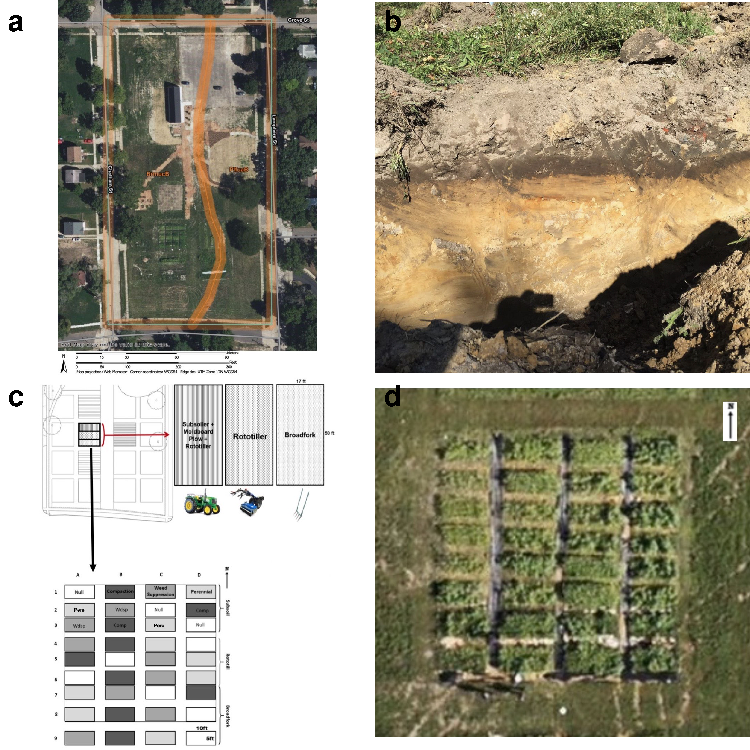
\includegraphics{merge_files/figure-latex/plots-1.pdf}

The soils can be classified as Technosols, given that large metal artifacts can be found throughout various profiles \emph{(\protect\hyperlink{ref-fao14}{FAO 2014})}, from when the area was filled in with nearby soils during highway road construction, as was common in mid-western USA industrial manufacturing cities many decades ago in the \emph{1960s} \emph{(\protect\hyperlink{ref-beniston16}{Beniston, Lal, and Mercer 2016})}.
Accordingly, the growing area has both a finer- and coarser-textured side \emph{(\protect\hyperlink{ref-USDA-NRCSwebsoilsurvey}{\textbf{USDA-NRCSwebsoilsurvey?}}--designPlots??)},
and this study was done on the side with consistent clay \textasciitilde37\% (\ref{fig:plots}).
Topsoil A horizons are 1-2'' (\textless5 cm) deep, and subsoil B horizons can be \textgreater30.5 cm (1 ft) deep, with a muted yellow color \emph{YR\#\#?!} (\ref{fig:plots}).
A baseline site-level soil lab assessment from Cornell determined that the top 4'' (10 cm) of soils around the site together have relatively good organic matter at \textasciitilde{} ± \% and nutrient levels, including those of heavy metals like lead and arsenic \emph{(Table ???)} which were present below harmful government human-contact standards \emph{(\protect\hyperlink{ref-angelone02}{\textbf{angelone02?}}; \protect\hyperlink{ref-EPA}{\textbf{EPA?}})}, as well as decent but sub-optimal \textasciitilde, CO, 2 respiration rates of ± mg per day (Table \ref{tab:chem}.
Some main concerns limiting productivity include high alkaline pH of 463.6 ± 24.9 lowering availability of existing nutrients, as well as weak aggregate stability of ± leading to issues with aeration, infiltration, rooting, crusting when dry, erosion, and runoff (Table \ref{tab:chem}).

\hypertarget{study-design}{%
\subsection{Study design}\label{study-design}}

The study area was a 278 \emph{m\textsuperscript{2}} (2992.4 \emph{ft\textsuperscript{2}}) section on the East side of the site that was divided into 36 separate 4.6 \emph{m\textsuperscript{2}} (49.5 \emph{ft\textsuperscript{2}}) plots in nine rows and four columns (Fig \ref{fig:plots}).
Tillage groups spanned the nine columns in adjacent groups of three, while cover crop mix treatments spanned the rows with one row per cover crop mix, which totaled 12 plots per tillage group and nine plots per cover crop mix.
Before applying treatments, approximately 0.2 \emph{m\textsuperscript{3}} (8.5 \emph{ft\textsuperscript{3}}) of compost was incorporated into each plot.

\emph{One aggregated sample per tillage group was collected and analyzed for chemistry using modified Morgan-extractable protocols at the MSU soil test lab (\protect\hyperlink{ref-moebius-clune16}{\textbf{moebius-clune16?}}) and analysis was also conducted on the compost.}

\hypertarget{tillage}{%
\subsection{Tillage}\label{tillage}}

These methods represent a spectrum of soil management practices used and potentially available for small scale agriculture.
Specifically we tested three tillage techniques:
1) no-till with a broadfork (NT),
2) moderate intensity with a roto-tiller (RT), and
3) intensive tractor-till (TT) with implements.
Tractor-till plots were worked with a subsoiler, moldboard plow, and rototiller attached to a tractor up to 30.5 cm (1 ft) deep.
RT plots were tilled with a rototiller implement up to 20 cm (7.9 in) deep.
NT plots were worked with a broadfork up to 10 cm (3.9 in) deep.
These treatments were selected based on varying tillage philosophies, costs of implementation, and degree of mechanization.

\hypertarget{cover-crop-mixes}{%
\subsection{Cover crop mixes}\label{cover-crop-mixes}}

Cover crop mixes were designed primarily based on plants associated with targeted benefits, and as possible, relative simplicity of re-seeding and winter-kill (e.g.~more heat tolerant) \emph{(\protect\hyperlink{ref-USDA15}{\textbf{USDA15?}})}.
We tested the performance of three mixes, each composed of three different plant species (Table \ref{tab:crops}).
The compaction mix focused on plants with roots that tend to penetrate and loosen soil well, specifically crimson clover (\emph{Trifolium incarnatum}), forage radish (\emph{Raphanus sativus}), and cereal ryegrass (\emph{Secale cereale}) \emph{(\protect\hyperlink{ref-williamsux2fweil04}{\textbf{williams/weil04?}})}.
The weed suppression mix consisted of heat- and drought-tolerant crops that grow rapidly, allowing them to outcompete other plants \emph{(\protect\hyperlink{ref-ref}{\textbf{ref?}})}, specifically sorghum-sudangrass (\emph{Sorghum bicolor x Sorghum bicolor var. sudanese}), cowpea (\emph{Vigna unguiculata subsp. unguiculata}), and buckwheat (\emph{Fagopyrum esculentum}).
Lastly, the perennial mix was made up of plants that would survive beyond one growing season and return in the spring, adding additional biomass and outcompeting early season weeds \emph{(\protect\hyperlink{ref-ref}{\textbf{ref?}})}, specifically hairy vetch (\emph{Vicia villosa}), red clover (\emph{Trifolium pratense}), and wheat (\emph{Triticum aestivum}).
We also had a null control group consisting of established vegetation within the plot, where no additional seeds were sown.

\begin{verbatim}
## ==  1 queries  ===============
## ✔  Found:  Hairy+Vetch[Common Name]
## ==  Results  =================
## 
## • Total: 1 
## • Found: 1 
## • Not Found: 0
## ==  1 queries  ===============
## ✔  Found:  Red+Clover[Common Name]
## ==  Results  =================
## 
## • Total: 1 
## • Found: 1 
## • Not Found: 0
## ==  1 queries  ===============
## ✔  Found:  Wheat[Common Name]
## ==  Results  =================
## 
## • Total: 1 
## • Found: 1 
## • Not Found: 0
## ==  1 queries  ===============
## ==  Results  =================
## 
## • Total: 1 
## • Found: 0 
## • Not Found: 0
## ==  1 queries  ===============
## ✔  Found:  Black-Eyed+Pea[Common Name]
## ==  Results  =================
## 
## • Total: 1 
## • Found: 1 
## • Not Found: 0
\end{verbatim}

\begin{table}

\caption{\label{tab:crops}Cover crop mixes}
\centering
\begin{tabular}[t]{l|l|l}
\hline
Function & Plants & Binomial\\
\hline
Null & Existing vegetation (no manipulation) & \\
\cline{1-2}
 & Hairy Vetch & \\
\cline{2-2}
 & Red Clover & \\
\cline{2-2}
\multirow{-3}{*}{\raggedright\arraybackslash Perennial} & Wheat & \\
\cline{1-2}
 & Forage Radish & \\
\cline{2-2}
 & Crimson Clover & \\
\cline{2-2}
\multirow{-3}{*}{\raggedright\arraybackslash Compaction} & Cereal Ryegrass & \\
\cline{1-2}
 & Sorghum-Sudangrass & \\
\cline{2-2}
 & Cowpea & \\
\cline{2-2}
\multirow{-3}{*}{\raggedright\arraybackslash Weed Suppression} & Buckwheat & \multirow{-10}{*}{\raggedright\arraybackslash NA}\\
\hline
\end{tabular}
\end{table}

\hypertarget{data-collection}{%
\subsection{Data Collection}\label{data-collection}}

\hypertarget{compaction}{%
\subsubsection{Compaction}\label{compaction}}

Soil compaction was measured with a penetrometer \emph{(AgraTronix, Soil Compaction Tester \#08180)} in four randomly selected spots within each quarter of every plot, which were later averaged at the plot level.
Individual measurements were recorded as the depth at which the penetrometer read 2 MPa (290.1) pounds per square inch or psi), since roots typically cannot penetrate with 2 MPa of force \emph{(\protect\hyperlink{ref-duiker02}{\textbf{duiker02?}})}.
Sampling was conducted at two separate time periods, in July (``Early'') and October (``Late'') 2019.
Samples were taken on dry days and recorded to the nearest inch.

\hypertarget{infiltration}{%
\subsubsection{Infiltration}\label{infiltration}}

We measured the water infiltration rate to determine the soil's capacity to drain water, which has implications for managing storm-water runoff and holding water for plant roots.
The infiltration rate was calculated by recording the amount of time it took for \textasciitilde1 L (32 fl oz) to drain into the soil, which is similar to the amount of typical rainfall on \textasciitilde0.10 \emph{m\textsuperscript{2}} (\textasciitilde1 \emph{ft\textsuperscript{2}}) per rain event \emph{(\protect\hyperlink{ref-USGS}{\textbf{USGS?}})}.
For each plot we cleared the soil surface of debris and cut vegetation low enough to explose the surface.
Then we pressed an empty \textasciitilde1.4 kg (48 oz) aluminum can \textasciitilde2.5 cm (1 in) into the soil and poured the water in.
The maximum time allowed was 160 seconds \textbf{recorded as\ldots??}.

\hypertarget{weed-cover-density-and-richness}{%
\subsubsection{Weed cover, density, and richness}\label{weed-cover-density-and-richness}}

We recorded three measures of weed activity that described overall weed pressure in different ways.
Weed cover was estimated as the proportion of total area covered by all weed species combined within a plot, using a scale of 1-10 with one indicating \textbf{only one species / near zero stems} observed to 10 being \textbf{10 species present / almost the entire plot surface covered at some level with at least part of a weed plant (e.g.~stem or leaf)}.
Weed richness was measured by counting the total number of morphologically distinguishable weedy plants with at least one individual stem observed in a plot.
Weed density was measured as the number of individual stems of either of the two most abundant weed species -- pigweed (\emph{Palmer amaranth / Amaranthus viridis}) and velvetleaf (\emph{Abutilon theophrasti}) -- using a discrete scale in increments of 10 with zero indicating neither species present and five indicating 50 or more total individuals stems of either species.

\hypertarget{yield}{%
\subsubsection{Yield}\label{yield}}

Five forage radish (\emph{Raphanus sativus}) roots were randomly selected from each plot and measured for length, individually, and wet weight, as a cluster.
The length of a radish root was measured from the hypocotyl, or root cap, to where the root became \textasciitilde6.3 mm (\textasciitilde1⁄4 in) wide.

\hypertarget{statistical-analyses}{%
\subsection{Statistical analyses}\label{statistical-analyses}}

All data were centered using plot-level medians and run through Kruskal-Wallis tests, which are non-parametric and make minimal assumptions about underlying distributions, making them relatively generalized and suitable for data with less replication.
Since these tests are limited in model formulation complexity, tests analyzing tillage and cover crop treatments were run separately, as reflected in the design of results figures.
In cases where a treatment category was significant overall, pairwise Wicoxon tests between all individual treatment pairs were run post-hoc to determine specific differences underlying the overall treatment effect, with Holm corrections to alpha levels and associated p-value adjustments for multiple comparisons, including alpha corrections to 0.01 when similar tests were run for independent sub-groups to uncover source of variation.
Data were also pooled across sample times given no preliminary significant effect on data, to increase statistical power under these statistical model conditions.
Finally, cover crop effects on yield were not analyzed, since yield data came from only compaction plots.
All calculations and analyzes were done in R version 4.2.0 (2022-04-22) mainly using the packages \emph{tidyverse} 1.3.1 \emph{(\protect\hyperlink{ref-tidyverse}{\textbf{tidyverse?}})}, \emph{rstatix} 0.7.0 \textbf{(\protect\hyperlink{ref-rstatix}{\textbf{rstatix?}})}, and \emph{ggpubr} 0.4.0 \emph{(\protect\hyperlink{ref-ggpubr}{\textbf{ggpubr?}})} \emph{compare\_means()} function.
Data and code are stored at \url{nmedina17.github.com/must}.

\hypertarget{results}{%
\section{Results}\label{results}}

\hypertarget{compaction-1}{%
\subsection{Compaction}\label{compaction-1}}

Compaction was affected significantly overall by tillage treatments (
\emph{H} = 38.2,
\emph{df} = 2,
\emph{n} = 72,
\emph{p} = \textless0.0001
) by
\textasciitilde52.4 \%
across cover crop treatments (Fig \ref{fig:compactFig}a).
Tractor-till had the largest significant effect on depth to hardpan compared to no-till (
\emph{p\textsubscript{adj}} = \textless0.0001
),
deepening the depth to hardpan by \textbf{\#\#} cm (conv\_, or \textasciitilde{}\emph{30-100}\%) compared to no-till,
down to
\textasciitilde20.6 ±
4.6 cm
(8.1 ±
1.8 in)
across all cover crop mixes.
Roto-till also had a marginally significant effect on depth to hardpan compared to no-till (
\emph{p\textsubscript{adj}} = 0.1
),
deepening the depth to hardpan by \textbf{\#\#} cm (conv\_, or \textasciitilde{}\emph{0-100}\%) compared to no-till, down to
\textasciitilde13.8 ±
1.9 cm
(5.4 ±
0.7 in).
The overall effect from tillage stemmed from significant effects among the perennial (
\emph{p\textsubscript{adj} = \textless0.01}
) and weed suppression (
\emph{p\textsubscript{adj} = \textless0.01}
) mixes (Fig \ref{fig:compactFig}a).
The effect of roto-till was more pronounced in the perennial mix (
\emph{p\textsubscript{adj} = \textless0.01}
), where depth to hardpan was about twice as deep as in no-till plots (Fig \ref{fig:compactFig}a).
There was also a significant difference of \textbf{\#\#\#} (conv\_, or \textasciitilde{}\emph{33}\%) between tractor- and roto-till among all cover crop mixes (Fig \ref{fig:compactFig}a).

\begin{figure}
\includegraphics[width=12.5in]{../figs/compactionPlot} \caption{Compaction data}\label{fig:compactFig}
\end{figure}

Compaction was not affected by cover crops among tillage groups overall (
\emph{H} = 2,
\emph{df} = 3,
\emph{n} = 72,
\emph{p} = 0.57
), but was significantly affected by cover crops specifically under no-till conditions (
\emph{Holm-corrected alpha = 0.01},
\emph{df = 3},
\emph{n = 6},
\emph{Wilcoxon p\textsubscript{adj} = \textless0.01}
) (Fig \ref{fig:compactFig}b).
Under no-till, the perennial mix had significantly shallower depth to hardpan compared to both null (
\emph{Holm-corrected alpha = 0.01, Wilcoxon p\textsubscript{adj} = \textless0.01}
) and weed suppression mixes (
\emph{Holm-corrected alpha = 0.01, Wilcoxon p\textsubscript{adj} = \textless0.01}
),
raising the depth to hardpan by
\textasciitilde{}\emph{5} cm (
2, or
\textasciitilde{}\emph{30-100}\%
) compared to each mix,
up to
\textasciitilde12.5 ±
7.4 cm
(
4.9 ±
2.9 in
) below the soil surface
(Fig \ref{fig:compactFig}b).

\hypertarget{infiltration-1}{%
\subsection{Infiltration}\label{infiltration-1}}

Soil infiltration was significantly affected by tillage (
\emph{H} = 8.5,
\emph{df} = 2,
\emph{n} = 48,
\emph{p} = 0.014
) but not cover crop mix (
\emph{H} = 5.9,
\emph{df} = 3,
\emph{n} = 48,
\emph{p} = 0.12
) (Fig \ref{fig:infilFig}).
Roto-till had significantly faster infiltration compared to no-till (
\emph{p\textsubscript{adj}} = 0
) and marginally significantly compared to tractor-till (
\emph{p\textsubscript{adj}} = 0.1
), speeding up infiltration by
\textasciitilde14.5 \%
compared to each tillage groups,
up to
\textasciitilde{} 13.4 ±
10.7 mL per sec
(
0.2 ±
0.2 in
)
(Fig \ref{fig:infilFig}a).

\begin{figure}
\includegraphics[width=12.5in]{../figs/infilPlot} \caption{Infiltration data}\label{fig:infilFig}
\end{figure}

\hypertarget{weed-pressure}{%
\subsection{Weed pressure}\label{weed-pressure}}

Weed density was overall marginally significantly affected by tillage (
\emph{H} = 6.5,
\emph{df} = 2,
\emph{n} = 72,
\emph{p} = 0.039
) by
\textasciitilde25.1 \%,
although weed cover (
\emph{H} = 0.2,
\emph{df} = 2,
\emph{n} = 36,
\emph{p} = 0.92
) and richness (
\emph{H} = 1.6,
\emph{df} = 2,
\emph{n} = 72,
\emph{p} = 0.44
) were not
(Fig \ref{fig:weedsFig}a).
Weeds under tractor-till were marginally significantly denser compared to no-till (
\emph{p\textsubscript{adj}} = 0.1
) and roto-till (
\emph{p\textsubscript{adj}} = 0.1
), denser by
\textasciitilde6.5 \%
compared to each tillage group,
up to
\textasciitilde{} 0.8 ±
0.2 \emph{stems per m\textsuperscript{-2}}
.

\begin{figure}
\includegraphics[width=12.5in]{../figs/weedPlot} \caption{Weeds data}\label{fig:weedsFig}
\end{figure}

All measured weed variables were affected significantly by cover crop mix, including
weed density (
\emph{H} = 20.1,
\emph{df} = 3,
\emph{n} = 72,
\emph{p} = 0.00016
) changing overall by
\textasciitilde6.5 \%,
weed cover (
\emph{H} = 10,
\emph{df} = 3,
\emph{n} = 36,
\emph{p} = 0.019
) changing overall by
\textasciitilde-5.5 \%, and
weed richness (
\emph{H} = 31,
\emph{df} = 3,
\emph{n} = 72,
\emph{p} = \textless0.0001
) changing overall by
\textasciitilde-0.5 \%
(Fig \ref{fig:weedsFig}b).
Weeds in the null mix covered significantly more plot area compared to the weed suppression mix (
\emph{p\textsubscript{adj}} = 0
) and marginally significantly compared to perennial (
\emph{p\textsubscript{adj}} = 0.1
) and compaction (
\emph{p\textsubscript{adj}} = 0.2
) mixes,
up to
\textasciitilde{} 4 ±
0 \%.
The null mix also had marginally significantly higher weed density compared to the weed suppression mix (
\emph{p\textsubscript{adj}} = 2e-04
) and marginally significantly compared to perennial (
\emph{p\textsubscript{adj}} = 0.2
) and compaction (
\emph{p\textsubscript{adj}} = 0.1
) mixes,
up to
\textasciitilde{} 0.9 ±
0.3 \emph{stems per m\textsuperscript{-2}}.
The weed suppression mix had the most detectable effects on both weed density and richness.
The weed suppression mix significantly lowered weed density compared to all other cover crop mix treatments, namely the null (
\emph{p\textsubscript{adj}} = 2e-04
), perennial (
\emph{p\textsubscript{adj}} = 0
), and compaction (
\emph{p\textsubscript{adj}} = 0.7
) mixes, by
\textasciitilde{} \textbf{\#\#} +-
\textbf{\#\#} (
conv\_, or
\textbf{\%\%\%}
), down to
\textasciitilde{} 0.4 ±
0 \emph{stems per m\textsuperscript{-2}}
.
The weed suppression mix also significantly lowered weed richness compared to all other cover crop mix treatments, namely the null (
\emph{p\textsubscript{adj}} = \textless0.0001
), perennial (
\emph{p\textsubscript{adj}} = \textless0.0001
), and compaction (
\emph{p\textsubscript{adj}} = 0.00093
) mixes, by
\textasciitilde{} \textbf{\#\#} +-
\textbf{\#\#} (
conv\_, or
\textbf{\%\%\%}
), down to
\textasciitilde{} 4 ±
1.5 morphoscpecies taxa
.

\hypertarget{yield-1}{%
\subsection{Yield}\label{yield-1}}

Radish yield was not significantly affected by tillage (
\emph{H} = 1.4,
\emph{df} = 2,
\emph{n} = 8,
\emph{p} = 0.5
), and centered at
\textasciitilde{} 13.2 ±
1.5 \emph{kg m\textsuperscript{-2}}
(
29.1 ±
3.3 \emph{lbs m\textsuperscript{-2}}
) and
\textasciitilde{} 0.1 cm
(
0 in
)
long (Fig \ref{fig:yieldFig}).

\begin{figure}
\includegraphics[width=12.5in]{../figs/yieldPlot} \caption{Yield data}\label{fig:yieldFig}
\end{figure}

\hypertarget{discussion}{%
\section{Discussion}\label{discussion}}

Overall this study informs urban soil management by supporting the use of tillage to address compaction issues and improve infiltration, together with cover crops to also reduce weed pressure.
Our hypothesis was partially supported, because overall tillage significantly deepened the depth to hardpan by \textasciitilde0.5 (Fig \ref{fig:compactFig}a), which was within the range of effect sizes measured among the various cover crop mixes within the no-till treatment (Fig \ref{fig:compactFig}b).
Additionally, infiltration was significantly affected by tillage, with roto-till showing the fastest rates (Fig \ref{fig:infilFig}a), which agreed with our predictions.
Furthermore, weed pressure was significantly affected by both cover crop mixes and tillage (Fig \ref{fig:weedsFig}), although effects from cover crop mixes, especially the weed suppression mix, were more widespread among multiple measured variables (Fig \ref{fig:weedsFig}b).
Despite these significant effects on soils, infiltration, and weeds, yields did not respond to tillage treatments.

\hypertarget{compaction-2}{%
\subsection{Compaction}\label{compaction-2}}

Short-term soil compaction issues are commonly alleviated by annual tilling \emph{(\protect\hyperlink{ref-ref}{\textbf{ref?}})}, and in addition to validating this practice, this study showed that cover cropping can also be used to manage compaction under no-till, although effects vary by mixture of taxa used.
Under tillage, this study validates that tillage intensity corresponds negatively with compaction (measured as depth to hardpan), and additionally clarifies that tractor-till can alleviate compaction in slightly deeper soils below main root zones under
\textasciitilde20.6 ±
4.6 cm
(8.1 ±
1.8 in),
as well as that roto-till can be useful under perennial crops, although under annuals, no-till can be just as effective as roto-till, saving grower time, energy, and cost for areas with crops harvested before rooting surpasses \emph{\textasciitilde10 cm (4 in)} \emph{(\protect\hyperlink{ref-krauseBlack95}{\textbf{krauseBlack95?}})}.
However for urban technosol soils, tilling can beneficially remove large metal artifacts and legacy construction debris like rebar, wires, cables, bricks, cinder blacks, and pipes, all of which could limit root growth under strict no-till management.
Tillage might also obscure cover crop effects on compaction, although cover crops may still provide other benefits, like soil macro-nutrients \emph{(\protect\hyperlink{ref-ref}{\textbf{ref?}})}.
Under no-till, this study found that perennial crop mixes can have significant effects on compaction, but rather than deep roots loosening soils in other studies \emph{(\protect\hyperlink{ref-ref}{\textbf{ref?}})}, in some cases depth to hardpan can instead become shallower.
This may be due to dense root mats that can form under grasses \emph{(\protect\hyperlink{ref-ref}{\textbf{ref?}})} like sorghum-sudangrass, which could further fill already limited pore space in densely-structured clay soils, helping water to pool under the soil surface \emph{(\protect\hyperlink{ref-ref}{\textbf{ref?}})}.
Overall other studies have found similar results \emph{(\protect\hyperlink{ref-OzpinarCay05}{\textbf{OzpinarCay05?}})}, suggesting short-term benefits of tillage to soil functions (yet long-term costs).

\hypertarget{infiltration-2}{%
\subsection{Infiltration}\label{infiltration-2}}

Water infiltration is a key function to improve urban soil functioning for agriculture by minimizing erosion and improving root available water, as well as mitigating storm-water runoff and flooding that often occurs after short heavy rains, due to soil sealing by concrete near hillslopes \emph{(\protect\hyperlink{ref-ref}{\textbf{ref?}})}.
This study found that roto-till resulted in significantly faster infiltration compared to no-till, unlike tractor-till, suggesting that roto-till management can generally be effective for improving infiltration and drainage.
This result could be explained by medium intensity roto-till increasing soil macro-porosity, which compared to soil micro-pores bind water less tightly allowing to flow faster \emph{(\protect\hyperlink{ref-ref}{\textbf{ref?}})}.
In contrast, the tractor diffused tillage energy across deeper soil volume, lowering the density of any added soil macro-pores and thereby making it easier for soil particles to settle back together, whereas no-till may have needed more time to improve macro-porosity via organic matter effects on soil structure \emph{(\protect\hyperlink{ref-king20}{\textbf{king20?}})}.
It is also possible that this result could be explained by compost incorporation, where tractor-till similarly incorporated compost more diffusely throughout the soil profile, diluting any compost benefits to infiltration.
Against a one inch rain event, this study supported the use of roto-till, but not no-till or tractor-till, which showed rates of only
\textasciitilde{} 6.2 ±
0 mL per sec
(
0.1 ±
0 gal per min
),
which would likely result in runoff pooling in roads and soil erosion.
Regarding cover crops, this study suggests that perennials may not have notable significant effects on infiltration rates, despite detectable effects on compaction.
Based on these findings, roto-till together with compost may be an effective strategy to improve urban soil water infiltration in the short-term, even if no-till may have more evidence as a longer-term strategy \emph{(\protect\hyperlink{ref-ref}{\textbf{ref?}})}.

\hypertarget{weed-suppression}{%
\subsection{Weed suppression}\label{weed-suppression}}

Weed suppression is important for reducing competition with crops as well as asthma and respiratory health risks from pollen \emph{(\protect\hyperlink{ref-katz14}{Katz and Carey 2014})}, and can also be achieved by tilling \emph{(\protect\hyperlink{ref-ref}{\textbf{ref?}})}, but this study additionally suggests that cover crops may be more likely to be effective.
Tractor-till, while able to combat relatively deep soil compaction, resulted in the highest weed density of the two most common weeds, velvet leaf (\emph{Abutilon theophrasti}) and pigweed (\emph{Palmer amaranth}), whose root density may have also slowed soil water infiltration rates.
This may have been due to fast-growing weed life histories taking advantage of looser soil, such as to re-sprout clonally \emph{(\protect\hyperlink{ref-ref}{\textbf{ref?}})}, and/or looser soil facilitating the establishment of weed seed banks.
However more notably, the targeted weed suppression mix of sorghum-sudangrass, buckwheat, and cowpea significantly reduced both weed density and richness by about half compared to the other cover crop mixes.
This result agrees with other studies pairing buckwheat and sorghum-sudangrass \emph{(\protect\hyperlink{ref-smith15}{Smith, Marín-Spiotta, and Balser 2015})}, and may have occurred due to competitive exclusion by sorghum-sudangrass and/or buckwheat via allelopathic chemical root defenses \emph{(\protect\hyperlink{ref-ref}{\textbf{ref?}})} or competition for light \emph{(\protect\hyperlink{ref-ref}{\textbf{ref?}})}, better phosphorus mining and use by buckwheat \emph{(\protect\hyperlink{ref-jabran17}{\textbf{jabran17?}}; \protect\hyperlink{ref-zhu02}{Zhu et al. 2002})}, facilitation or amplification of these previous effects by cowpea's added nitrogen supply \emph{(\protect\hyperlink{ref-ref}{\textbf{ref?}})}, and/or existing adaptations to poor dry soils \emph{(\protect\hyperlink{ref-ref}{\textbf{ref?}})} allowing high biomass accumulation.
Given both effectiveness and relative ease of re-seeding and winter-kill, this weed suppression mix can be used to frame crop beds, keeping out encroaching weeds, or to reduce weed pressure in an area that might be planted in the fall or following season.

\hypertarget{yield-2}{%
\subsection{Yield}\label{yield-2}}

Despite overall significant effects by tillage on compaction, infiltration, and weeds, tillage did not significantly affect radish yield.
As is, this study does not rule out more complex relationships between soil compaction, infiltration, and crop yield, as suggested by other studies \emph{(\protect\hyperlink{ref-ref}{\textbf{ref?}})}.
However, with more statistical replication, it is possible that no-till would show slightly higher yields, validating similar studies \emph{(\protect\hyperlink{ref-refs}{\textbf{refs?}})} pointing to more fundamental soil structure and microbial benefits under no-till.
Overall yields tend to respond more to longer-term reservoirs of water and nutrients like mulched compost compared to shorter-term, transient influxes brought by infiltration processes \emph{(\protect\hyperlink{ref-schlegelHavlin17}{\textbf{schlegelHavlin17?}})}.
As a result, it is possible that similar alternative soil management practices like no-till combined with compost and mulching application may lead to better yields.
Additionally, other studies suggest that forage radish can be an effective cover crop in reducing compaction and building soil structure, with minimal or no mechanical tillage \textbf{(\protect\hyperlink{ref-chen10}{Chen, Tam, and Ye 2010})}.
However ultimately this study suggests the need for future studies of processes tying yield to land management strategies particularly in similar urban clay soils with legacy compaction and pH concerns.

\hypertarget{conclusion}{%
\subsection{Conclusion}\label{conclusion}}

Taken together, this study presents data that, in addition to validating previous studies supporting general tillage for short-term soil fertility, also validates the use of medium-intensity roto-till and cover crop mixtures specifically for weed suppression.
This study serves as a model demonstration of both widely accessible and effective strategies for growing on re-purposed urban soils after urban land-use turnover.
We advocate for the maximal use of cover crop mixes for various target functions, with medium-intensity tillage to jump-start urban cultivation.

\newpage

\hypertarget{references}{%
\section*{References}\label{references}}
\addcontentsline{toc}{section}{References}

\hypertarget{refs}{}
\begin{CSLReferences}{1}{0}
\leavevmode\vadjust pre{\hypertarget{ref-beniston16}{}}%
Beniston, Joshua W., Rattan Lal, and Kristin L. Mercer. 2016. {``Assessing and {Managing Soil Quality} for {Urban Agriculture} in a {Degraded Vacant Lot Soil}: {ASSESSING AND MANAGING SOIL QUALITY FOR URBAN AGRICULTURE}.''} \emph{Land Degradation \& Development} 27 (4): 996--1006. \url{https://doi.org/10.1002/ldr.2342}.

\leavevmode\vadjust pre{\hypertarget{ref-chen10}{}}%
Chen, G. C., N. F. Y. Tam, and Y. Ye. 2010. {``Summer Fluxes of Atmospheric Greenhouse Gases {N2o}, {Ch4} and {Co2} from Mangrove Soil in {South China}.''} \emph{Science of The Total Environment} 408 (13): 2761--67. \url{https://doi.org/10.1016/j.scitotenv.2010.03.007}.

\leavevmode\vadjust pre{\hypertarget{ref-fao14}{}}%
FAO. 2014. \emph{World Reference Base for Soil Resources 2014: International Soil Classification System for Naming Soils and Creating Legends for Soil Maps}. {Rome}: {FAO}.

\leavevmode\vadjust pre{\hypertarget{ref-katz14}{}}%
Katz, Daniel S. W., and Tiffany S. Carey. 2014. {``Heterogeneity in Ragweed Pollen Exposure Is Determined by Plant Composition at Small Spatial Scales.''} \emph{Science of the Total Environment} 485--486 (1): 435--40. \url{https://doi.org/10.1016/j.scitotenv.2014.03.099}.

\leavevmode\vadjust pre{\hypertarget{ref-kumar16}{}}%
Kumar, Kuldip, and Lakhwinder S. Hundal. 2016. {``Soil in the {City}: {Sustainably Improving Urban Soils}.''} \emph{Journal of Environmental Quality} 45 (1): 2--8. \url{https://doi.org/10.2134/jeq2015.11.0589}.

\leavevmode\vadjust pre{\hypertarget{ref-kuzyakov19}{}}%
Kuzyakov, Yakov, and Kazem Zamanian. 2019. {``Reviews and Syntheses: {Agropedogenesis} \textendash{} Humankind as the Sixth Soil-Forming Factor and Attractors of Agricultural Soil Degradation.''} \emph{Biogeosciences} 16 (24): 4783--803. \url{https://doi.org/10.5194/bg-16-4783-2019}.

\leavevmode\vadjust pre{\hypertarget{ref-montgomery07}{}}%
Montgomery, David R. 2007. {``Soil Erosion and Agricultural Sustainability''} 104 (33): 13268--72.

\leavevmode\vadjust pre{\hypertarget{ref-oldfield19}{}}%
Oldfield, Emily E., Mark A. Bradford, and Stephen A. Wood. 2019. {``Global Meta-Analysis of the Relationship Between Soil Organic Matter and Crop Yields,''} 15--32.

\leavevmode\vadjust pre{\hypertarget{ref-small19}{}}%
Small, Gaston, Paliza Shrestha, Geneviève Suzanne Metson, Katherine Polsky, Ivan Jimenez, and Adam Kay. 2019. {``Excess Phosphorus from Compost Applications in Urban Gardens Creates Potential Pollution Hotspots {Excess} Phosphorus from Compost Applications in Urban Gardens Creates Potential Pollution Hotspots.''}

\leavevmode\vadjust pre{\hypertarget{ref-smith15}{}}%
Smith, A. Peyton, Erika Marín-Spiotta, and Teri Balser. 2015. {``Successional and Seasonal Variations in Soil and Litter Microbial Community Structure and Function During Tropical Postagricultural Forest Regeneration: {A} Multiyear Study.''} \emph{Global Change Biology} 21 (9): 3532--47. \url{https://doi.org/10.1111/gcb.12947}.

\leavevmode\vadjust pre{\hypertarget{ref-stewart07}{}}%
Stewart, Catherine E., Keith Paustian, Richard T. Conant, Alain F. Plante, and Johan Six. 2007. {``Soil Carbon Saturation: Concept, Evidence and Evaluation.''} \emph{Biogeochemistry} 86 (1): 19--31. \url{https://doi.org/10.1007/s10533-007-9140-0}.

\leavevmode\vadjust pre{\hypertarget{ref-zhu02}{}}%
Zhu, Y. G., Y. Q. He, S. E. Smith, and F. A. Smith. 2002. {``Buckwheat ({Fagopyrum} Esculentum {Moench}) Has High Capacity to Take up Phosphorus ({P}) from a Calcium ({Ca})-Bound Source.''} \emph{Plant and Soil} 239 (1): 1--8. \url{https://doi.org/10.1023/A:1014958029905}.

\end{CSLReferences}

\end{document}
